\scanpage{80}
\mspage{79}%
valente à $\handwritten{\underline}{G}(\handwritten{\ell})$ pour tout corps alg. clos $\handwritten{\ell}$ de ca\rlap{\raisebox{-.65em}{r}}r. $p\handwritten{>0}$ (de façon précise, si $\handwritten{\overline}{\handwritten{\underline}{F}}_p$ est\deleted{\unsure{l|t}} la clôture algébrique de $\handwritten{\underline}{F}_p$ dans $\handwritten{\ell}$, l'inclusion de celle-ci dans $\handwritten{\ell}$ ind\rlap{i}uit une équivalence de \unsure{g|\rlap{e}g}erbes
\[
\handwritten{\underline}{G}(\handwritten{\ell})\handwritten{\underline{\approx}}\handwritten{\underline}{G}(\handwritten{\overline}{\handwritten{\underline}{F}}_p)\deleted{\handwritten{\unsure{)|,}}}\handwritten{\underline{\approx}}\handwritten{\underline}{H}\deleted{\handwritten{\unsure{)|.}}}\qquad ).
\]
8.6. Etude de $\operatorname{Rep}(\handwritten{\underline}{H})$. Nous avons dit que les classes d'objets simples sont en correspondance biunivoque avec les éléments de $\handwritten{\underline}{Q}$ ; l'élément de $\handwritten{\underline}{Q}$ correspondant à un objet isotypique est \unsure{\rlap{e}d|d}it la \handwritten{\uline}{pente} de cet élément. Nous avons vu que l'objet de $\operatorname{Rep}(\handwritten{\underline}{H})$ défini \margin{\handwritten{Notation $E_{s/r}$ pour $E_{r,s}$ indiquée, donc
\[
E_\lambda\otimes E_{\lambda'}\simeq E_{\lambda\lambda'}^{n(\lambda,\lambda')}
\]
pour $\lambda,\lambda'\in\mathbb{Q}$}}
par l'objet $\handwritten{\underline}{Q}_p[T]/(T^r-p^s)$ de $\operatorname{Fcriso}(\handwritten{\underline}{F}_p)$, muni de la multiplication par $T$, est simple de pente $s/r$ ($s,r\handwritten{\in}\handwritten{\underline}{Z}$, $r\geq1$, $(s,r)=1$ ), de sorte que nous obtenons ainsi un catalogue complet des objets simples $E_{r,s}$. Bien entendu, $E_{r,s}$ est de rang $r$, d'autre part son corps des endomorphismes est \deleted{\unsure{lta|ila}} un corps gauche \inserted{$K_{r,s}$}\handwritten{\begin{tikzpicture}[baseline=0cm,x=1cm,y=1cm]\draw[thin] (0,0) .. controls (.35,.16) and (.7,.1) .. (1.05,.08) .. controls (1.45,.05) and (1.6,.22) .. (1.64,.48);\end{tikzpicture}} dont la classe dans $\operatorname{Br}(\handwritten{\underline}{Q}_p)=\handwritten{\underline}{Q}/\handwritten{\underline}{Z}$ est $s/r\bmod1$, d'après ce qu'on a vu dans 8.3.

$\operatorname{Rep}(\handwritten{\underline}{H})$ est limite inductive des sous-c\unsure{\rlap{q}a|a}tégories pleines $\operatorname{Rep}(\handwritten{\underline}{H},r)$, $r\geq1$, où $(\handwritten{\underline}{H},r)$ est le quotient de la gerbe $\handwritten{\underline}{H}$ correspond au quotient $(H,r)$\handwritten{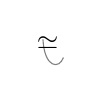
\begin{tikzpicture}[baseline=-.1cm,x=1cm,y=1cm]\draw[gray,thin] (.22,.15)..controls (.24,-.22) and (.43,-.23)..(.48,-.08);\node at (.28,.1) {$\simeq$};\end{tikzpicture}}$\handwritten{\underline}{G}_m$ de son lien, tel que l'homomorphisme de Tate \deleted{soit un} induise un homomorphisme $(H,r)\handwritten{\xrightarrow{\unsure{q|a|\alpha}}}\handwritten{\underline}{G}_m$ s'identifiant à $x\handwritten{\longmapsto}x^r$ : F-iso\inserted{cristaux (sur $\handwritten{\overline}{k}$) de pente multiple de $1/r$.}\handwritten{\begin{tikzpicture}[baseline=0cm,x=1cm,y=1cm]\draw[thin] (0,-.17)..controls (.16,.05) and (.35,.02)..(.62,.02)..controls (.85,.03) and (.95,.08)..(1.05,.12);\end{tikzpicture}} Donc $(\handwritten{\underline}{H},r)$ \deleted{s'identifie} \unsure{\rlap{a}è|è}s\unsure{\rlap{l}t|t}\deleted{\unsure{a|à}} \inserted{une}\handwritten{\begin{tikzpicture}[baseline=0cm,x=1cm,y=1cm]\draw[thin] (0,-.13)--(.65,.13);\end{tikzpicture}} gerbe de lien $\handwritten{\underline}{G}_m$, ayant comme classe dans $\operatorname{Br}(\handwritten{\underline}{Q}_p)$ l\unsure{\rlap{i}e|e} générateur canonique $1/r\bmod\handwritten{\underline}{Z}$ de ${}_r\operatorname{Br}(\handwritten{\underline}{Q}_p)\handwritten{\simeq}\handwritten{\underline}{Z}/r\handwritten{\underline}{Z}$. C\rlap{,}'est aussi, plus canoniquement, ``la'' gerbe définie par le corps gauche $K_{r,\handwritten{1}\deleted{s}}$ plus haut, \deleted{qui}

\handwritten{[}Exercice amusant, que je n'ai pas fait: la structure additive de $\operatorname{Rep}(\handwritten{\underline}{H})$ étant entièrement décrite par la collection de\unsure{s|\rlap{z}s} $K_{r,s}$, expliciter sa $\handwritten{\otimes}$-structure ... i.e. écrire les \handwritten{``}relations canoniques\handwritten{''} en termes de prod\unsure{\rlap{n}u|u|n}i\unsure{\rlap{e}t|t|e}s tensoriels entre les $E_{r,s}$. Autre exerciee suggéré: trouver ``canoniquement'' une description des modules de Dieudonné des réduits des groupes de Lubin-Tate en termes des $E_{r,s}$ \deleted{\handwritten{\unsure{;|,|.}}} \handwritten{(}en particulier, les Lubin-Tate associés aux extensions non ramifiées

